
\documentclass[journal]{IEEEtran}
%% Enable Latin characters
\usepackage[utf8]{inputenc}
% If IEEEtran.cls has not been installed into the LaTeX system files,
% manually specify the path to it like:
% \documentclass[journal]{../sty/IEEEtran}

\hyphenation{op-tical net-works semi-conduc-tor}

\usepackage[square,numbers,sort&compress]{natbib}

%% Acronyms
\usepackage[nolist]{acronym}

%% Better equations
\usepackage{amsmath, amsthm, amssymb, amsfonts}
%% Better figures
\usepackage[caption=false,font=footnotesize]{subfig}
\usepackage{fixltx2e}
\usepackage{graphics}
\usepackage{epsfig}

\usepackage{hyperref}

%% Pseudo-code algorithms
\usepackage{setspace}
\usepackage[ruled,vlined]{algorithm2e}

%% better verbatim
\usepackage{fancyvrb}

\begin{document}
%
% paper title
% can use linebreaks \\ within to get better formatting as desired
% Do not put math or special symbols in the title.
\title{Homophilic Self Organizing Feature Maps:\\ Topic Detection on Socially Connected Data}

\author{Bernardo Carvalho Simões \\Instituto Superior Técnico \\ bernardo.simoes@ist.utl.pt}

% make the title area
\maketitle

% As a general rule, do not put math, special symbols or citations
% in the abstract or keywords.
\begin{abstract}
With the evolution of social media platforms, the amount of unlabeled information has gone skyrocketing, the process of labeling this kind of information evermore complex. Typical approaches used on the WEB for Topic Detection and Tracking cannot be directly applied due to the small amount of text produced per tweet, orthographic errors, abbreviations and so on.

We propose and analyze a new form of topic detection and tracking on social networks. By leveraging the social relations between authors of the gathered content, and apply them to the clustering process.

In order to achieve this, we proposed some modifications to the artificial neural network  and clustering algorithm --- Self Organizing Maps. 
\end{abstract}

% Note that keywords are not normally used for peerreview papers.
\begin{IEEEkeywords}
topic detection, twitter, self-organizing maps, classification, clustering
\end{IEEEkeywords}

\section{Introduction}
\IEEEPARstart{F}{inding} topic sensitive information on social networks is extremely complicated due to the fact that documents have very little content, slang vocabulary, orthographic mistakes and abbreviations. \citet{Asur2010} successfully predicted box-office revenues by monitoring the rate of creation of new topics based on debuting movies. Their work outperformed some traditional market-based predictors.

Thus, academic and enterprise worlds started looking at \ac{ML} for new ways to achieve revenue or simply explore and discover patterns in data. 

Using unsupervised \ac{ML}, \citet{Le2011} was able to achieved 81.7\% accuracy in detecting human faces, 76.7\% accuracy when identifying human body parts and 74.8\% accuracy when identifying cats. 

Social Media Analytics is another raising topic that draws from Social Network Analysis~\cite{knoke2008social}, \ac{ML}, Data Mining~\cite{witten2005data}, \ac{IR}~\cite{salton1983introduction}, and \ac{NLP}. As stated~\citet{Melville2009}, 32\% of the 200 million active bloggers write about opinions on products and brands, while 71\% of 625 million Internet users read blogs and 78\% of respondents put their trust in the opinion of other consumers. In comparison, traditional advertising is only trusted by 57\% of consumers.
This kind of data drives companies to Social Media Analytics as a way to know what people are saying on the web about their companies and products. This new worry has brought to life a lot of new startups like Sumalor ThoughtBuzz, but also solutions from the old players like IBM and SAS.

The main objective of this project is to find topics on tweets by contextualizing the social network involving the person that authored the tweet in the clustering process.

We start by building a dataset, in order to train the \ac{SOM}, that will later classify each future tweet that arrives on the network.

After creating the dataset, we will try to find clusters of topics using the default \ac{SOM} approach, converting each tweet to \ac{VSM}. After analyzing the results from the default \ac{SOM} approach, the algorithm will be changed in order to give relevance to the social relationship between authors of tweets.

\section{Related Work}
\label{sec:related_work}

\subsection{Clustering with Self-Organizing Maps} 
\label{sec:the_self_organizing_map}

\subsubsection{The Self-Organizing Map} 
\label{subsubsec:the_self_organizing_map}
\ac{SOM} are a two layer recurrent \ac{ANN} that has the desired property of topology preservation, thus mimicking the way cortex of highly developed animal brains work. \ac{SOM} allow cluster visualization of multi-dimensional data, similar to methods such as \ac{MDS}~\cite{KruskalWish1978} and \ac{PCA}~\cite{Hotelling_1933} .  

\citet{Bacao2005} described the basic idea behind \ac{SOM} as a mapping between input data patterns into a n-dimensional grid of neurons, or units. That grid is also know as the output space, as opposed to the initial space --- input space --- where the input patterns reside. An illustration of both spaces can be seen in Figure~\ref{fig:5_neighbours_converge}.

SOMs work in a similar way as is thought the human brain works. Analogously to the human brain, SOMs also have a set of neurons that, through learning experience, specialize in the identification of certain types of patterns. These neurons are responsible for categorizing the input patterns for which they are responsible to identify. Nearby neurons will be organized by similarity, which will cause similar patterns to activate similar areas of the \ac{SOM}.
With this topology preserving mapping, the \ac{SOM} organizes information spatially, where similar concepts are mapped to adjacent areas. The topology is preserved in a sense that, as far as possible, neighborhoods are preserved throughout the mapping process.
Output neurons are displayed in an n-dimensional grid, generally rectangular, but other structures are possible, such as hexagonal or octagonal.  The grid of neurons, in the output space, can be divided in neighborhoods --- where neurons responsible for the same kind of input reside.
In \ac{SOM}, neurons will have the same amount of coefficients as the input patterns and can be represented as vectors.

Before describing the algorithm, it is important to define two key aspects of the \ac{SOM}: the learning rate and the quantization error. The learning rate is a function that will be decreased to converge to zero. It will be applied to winning neurons and their neighbors in order for them to move toward the corresponding input pattern in progressively smaller steps. Quantization error is the distance between a given input pattern and the associated winning neuron. It describes how well neurons represent the input pattern. The radius of the neighborhood around the winning neuron is also particularly relevant to the topology of the \ac{SOM}, deeply affecting the unfolding of the output space as stated by~\citet{Bacao2005}. 

%SOM training is always subject to some variability due to multiple causes, like the sensitivity of initial conditions, convergence to local minima and sampling variability~\cite{Bodt}.

%No general formula exists to minimize quantization error~\cite{Bodt} . In order to achieve a minimal value, the number of neurons, value of neurons and order of the input data is randomly changed. Multiple SOMs are trained and the one with the lowest mean quantization error is chosen.

In order to know how well a neuron maps to all the input patterns it represents, the average of the quantization error can be used(Eq. \ref{eq:avg_quant_error}). On the equation, $d_{i,n}$ is an input pattern that is represented by the neuron $w$. Each neuron represents an arbitrary number --- $n$ --- of input patterns. That group of input patterns is represented as $D_{i,j}$.
\par

\begin{equation}
  \label{eq:avg_quant_error}
  \varepsilon(w) = \frac{\sum_{i=0}^{n} \| w - d_{i}  \| }{n}, d_{i} \in D, \forall n
\end{equation} 

% Self Organizing Map algorithm in latex, needs package algorithm2e
  \begin{algorithm}
    \label{alg:som}
    \DontPrintSemicolon
    \KwData{Input patterns $X = \{  \overrightarrow{x_1}$,\dots,$\overrightarrow{x_N}$ \}, number of iterations $t_{\textrm{$max$}}$,  neighborhood function $\sigma(t)$, learning rate  $\epsilon(t)$ }
    \KwResult{Trainned map and clustered input patterns}
    Randomly initialize neurons, $w_i \in \mathbb{R}^{D}, \forall i $ \;
    \For{ $t = 1 \; to \; t_{\textrm{$max$}}$ }{
      Randomly draw an input pattern, $ \overrightarrow{x_d} $  \;
      \nl\label{som:one}$p =  \arg{ min_i \{ \|  \overrightarrow{x_d} - \overrightarrow{w_i} \|  \}}  $  \;
      \nl\label{som:two}$\overrightarrow{w_i} = \overrightarrow{w_i} + \epsilon(t) \cdot h_{ip}(t) \cdot ( \overrightarrow{x_d} - \overrightarrow{w_i} ),  \forall{i}$ \;
      \nl\label{som:three}$\sigma(t) = \sigma_0( \sigma_f / \sigma_0 )^{t/t_{max}}$  \;
      \nl\label{som:four}$\epsilon(t) = \epsilon_0( \epsilon_f / \epsilon_0 )^{t/t_{max}}$ \;  
      \nl\label{som:fifth}$ t \leftarrow t + 1$}
      \caption{Self-Organizing Map \cite[]{Kohonen1990} }
  \end{algorithm}

The learning phase is characterized by the Algorithm~\ref{alg:som}, which works the following way:
\begin{itemize}
  \item \textbf{On line 1:} The neuron closer to the input pattern is selected. The Euclidean distance (Eq.~\ref{eq:eucl_dist}) is generally used.
    \begin{equation}
  \label{eq:eucl_dist}
  Dist=\sqrt{\sum_{i=0}^{i=n}( V_i-W_i)^2}
\end{equation} 

  \item \textbf{On line~\ref{som:two}:} the winning neuron $(p)$ previously selected on line 1 is updated, in order to better represent the input pattern. Also, all other neurons inside a specific radius will also be updated --- this process is described in Figure~\ref{fig:5_neighbours_converge}. Each neuron is updated with a different rate of influence determined by how far away it is from the winning neuron, which is defined by the neighborhood influence function $h_ip(t)$. The Gaussian (Eq.~\ref{eq:gaussian}) is often used. 
    \begin{equation}
  \label{eq:gaussian}
  h_{ip}(t)=\exp{-\frac{|\overrightarrow{a_i}-\overrightarrow{a_p}|^2}{\sigma^2(t)}}
\end{equation} 

  \item \textbf{On line~\ref{som:three}:} the size of the radius will be updated.
  \item \textbf{On line~\ref{som:four}:} the learning rate is updated.
  \item \textbf{On line~\ref{som:fifth}:} the number of iterations is incremented.
\end{itemize}
 
In order for the algorithm to converge, the learning rate and the radius of the neighborhood need to decrease at a given rate. This process can be seen on line \ref{som:three} and \ref{som:four}, respectively .
%Generally exponential decay is used.

\begin{figure}
  \begin{center}
    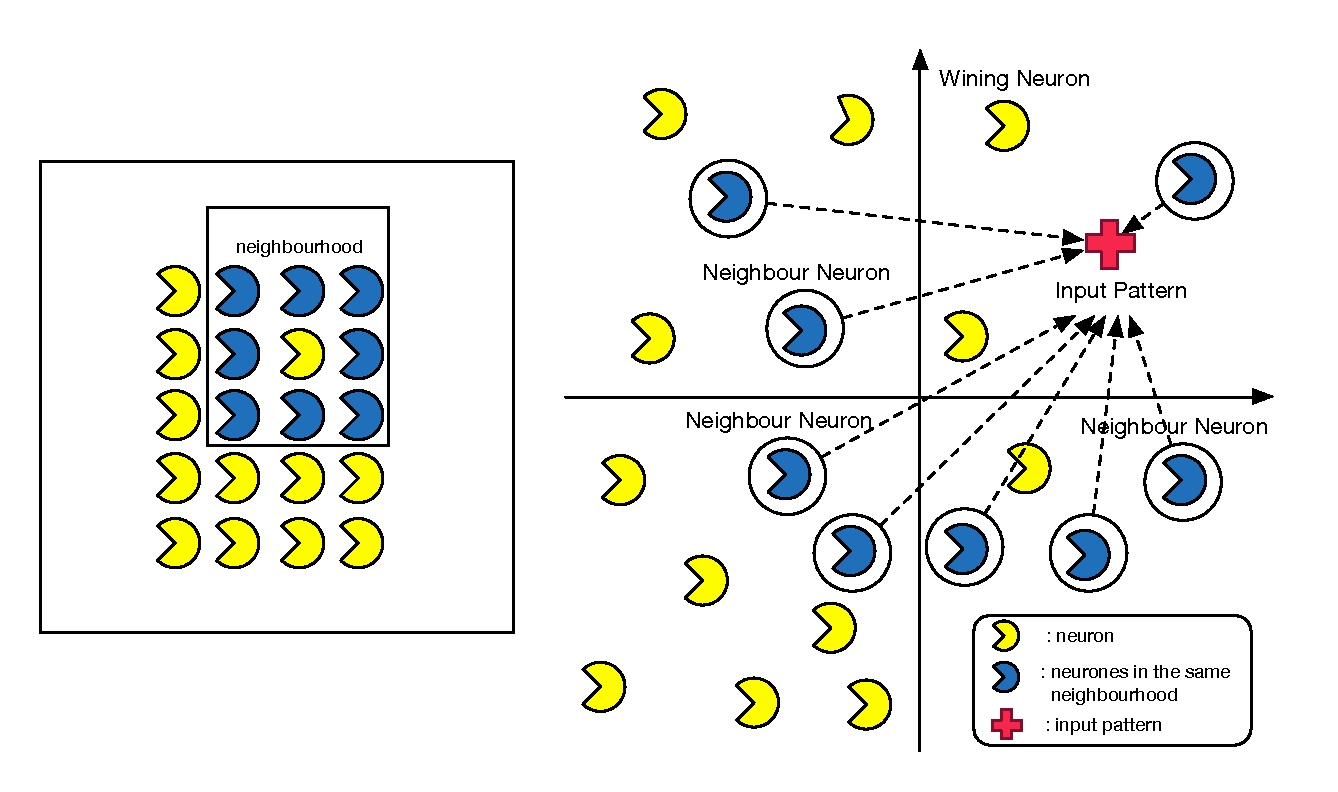
\includegraphics[width=7cm]{images/5_neighbours_converge.eps}
  \end{center}
  \caption{ On the left the output space neighborhood, on the right the neighbors of the winning neuron converging in the direction of the input pattern }
  \label{fig:5_neighbours_converge}
\end{figure}

The prediction phase can start after the model is learned. On the prediction phase, new input patterns can be quickly assigned to the \ac{SOM}, without need to apply the learning rate to the winning neuron and his neighbors. In other words, only line 1 will run. Due to the fact that the input pattern will be assigned to the cluster that is mapped by the nearest neuron. Thus, it is very easy and fast to classify new data now. As stated by ~\citet{Liu2012b}, the advantages of using \ac{SOM} are: data noise immunity, easy to visualize data, and parallel processing.

In order to visually interpret the result of the \ac{SOM}, \ac{U-Matrix} method may be used~\citep{Bacao2005}. The \ac{U-Matrix} is a representation of the \ac{SOM}, in which the distance between neurons is represented in a gray-scale where the darkest colors represent the farthest distance and the lightest colors the closer neurons.

\subsubsection{The Geo-SOM} 
\label{sub:types_of_soms}
The Geo-SOM, by~\citet{Bacao2005}, applies the first law of geography “Everything is related to everything else, but near things are more related than distant things."~\cite{citeulike:612692} to the \ac{SOM} algorithm. In this case, the winning neuron is chosen in a radius defined by the geographic-coordinates of the data, forcing units that are close geographically to be close in the output space.

The algorithm works by defining a variable $k$ which is used as a "geographical tolerance" that forces the winning neuron to be geographically near the input pattern. When $k=0$, the winning neuron is forced to be the unit geographically closest to the input data, whilst $k$ increases, the tolerance for data with further geographic coordinates, increases as well. $k$ is a geographic radius applied in the output space. When the radius exceeds the size of the output space, every unit is eligible to be the winning neuron, and therefor, we have a regular \ac{SOM}.

The selection of the winning neuron is done in two steps. First, geographic neurons inside the tolerance $k$ with the input data as a center are selected. Only after that, comparisons are made with the rest of data present in the input data. The representation of the Geo-SOM can be seen in Figure~\ref{fig:geo_som}, where the units considered for the best match are defined by a sort of geographic radius defined by $k$, whilst in the original \ac{SOM}, the winning neuron could have been any of the units presented on the figure.

The Geo-SOM approach to the alteration of the default \ac{SOM} algorithm is specially interesting due to the fact that this thesis objective is also to give relevance to data patterns that are not located in the same space as the trained data. In a way, what we are trying to achieve is similar to the work by~\citet{Bacao2005} but changing the geographic relevance in data by a social relevance.
\begin{figure}[tb]
  \begin{center}
    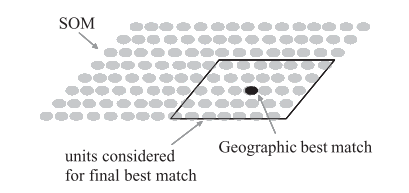
\includegraphics[width=0.8\linewidth]{images/6_geo-som.png}
  \end{center}
  \caption{Geo-SOM structure, where the units considered to be the winning neuron are constrained by the geographic coordinates of the data, from~\citet{Bacao2005}}
  \label{fig:geo_som}
\end{figure}

\subsubsection{WEBSOM}
\label{sub:websom}
\citet{honkelawebsom} developed a new approach to automatically order arbitrary, free from textual, document collections, using two different SOMs. The first \ac{SOM} is called word category map and it's used to find words that have similar meaning, while the second \ac{SOM}, called document map, is the one actually used to cluster the documents. 

The WEBSOM was not based on keywords and boolean expressions, instead, words with the same meaning are encoded in a word category map, where placement and frequency in documents is taken into account. This way it is possible to remove words with similar meaning --- greatly reducing the \ac{VSM} size  making it possible to train the document map in a scalable way.
                                                                                                          
\subsection{Twitter Data Mining and TTD} 
\label{sec:data_mining_in_twitter_}

In this subsection, we will focus on work done on the Twitter social network in order to leverage insights on how the public data available from the website can be explored. 

\subsubsection{Topic and Trending Detection} 
\label{sub:real_time_topic_and_trending_detection}

~\citet{allan2002topic} defined \ac{TDT} as “a constantly arriving stream of text from newswire and from automatic speech-to-text systems that are monitoring selected television, radio, Web broadcast news shows. Roughly speaking, the goal of \ac{TDT} is to break the text down into individual news stories, to monitor the stories for the events that have not been seen before, and to gather stories into groups that each discuss a single news topic".

Nowadays, due to the rapid adaptation of people to always be on-line, through the usage of cellphones on the move, desktops at work and even TV at home, the increase of user generated content has increased tremendously in latest years. In 2006, 35\% of on-line adults and 57\% of teenagers created content on the Internet \footnote{ Data source: http://www.pewinternet.org/Presentations/2006/UserGenerated-Content.aspx}, which in "Internet Years" was ages ago. 

The challenge of \ac{TDT} is evermore focused on online generated documents, and in new forms to be able to track and categorize all the information that is continuously being generated.
Many \ac{TDT} techniques have been proposed,  a significant amount of them rely on the \ac{TF-IDF}~\cite{Baeza-Yates:1999:MIR:553876}. Because tweets are very small, often with typos or slang words, and because the same tweet might be written in multiple languages, \ac{TF-IDF} is not particularly adequate for topic detection on twitter. In this subsection, we will take a look at multiple methods of topic detection in general, and also specifically on the Twitter social network.

~\citet{Cataldi2010} proposed a new technique for emerging topic detection that permits real-time retrieval of the most emergent topics expressed by a community on Twitter. Their work applies the PageRank algorithm~\cite{Pagerank1998} to the users follower/followee relationship, in order to find the most influential users on the network. Then, the most trending topics are calculated, by relating social influence, word co-occurrence and time frame. In the end, an interface was created where it would be possible to navigate, through hot topics in a given time frame. Topic labeling was not automatic and was implicit by the time frame of an event.

~\citet{Weng2010} also used the PageRank algorithm to find the most influential twitter users on a certain topic. However, using a different approach, they represent each twitter user as a bag of words comprising of all the tweets that they have posted, and applied \ac{LDA}~\cite{Blei2003} in order to find topics in which users are interested in. Finally, it was possible to prove that follower/followee relations on twitter are not just casual, but that people actually follow other people to whom they have some resemblance or common interest. This concept is called homophily and will be further explored on this thesis.
                                                                                                          \subsubsection{Tweeter Natural Language Processing}
\label{sub:tweeter_natural_language_processing}
Using standart \ac{NLP} tools on tweets has been extremely unreliable, due to the fact that microbloging text tends to be full of abbreviations, emojis and smiles . Recently, ~\citet{owoputi13improvedparth} published a \ac{NLP} library, specific for twitter. ARK Tweet \ac{NLP} can tag words that are only used in social networks. The tagger was built using maximum entropy Markov model, where a tag is assigned to a word based on the entire tweet text, and the tag assigned to the word to its left. ~\citet{owoputi13improvedparth} state that the tagger has a 93.2\% accuracy. 
By using \ac{NLP} tools, it is possible to reduce the dimension of \ac{VSM} space by only choosing words that are relevant, like common nouns, hashtags and proper nouns. This will not only yield better results by removing tweets that have no content, and therefor, cannot be categorized, but will also increase performance during training due to the reduced dimensions caused by less use of words.
 
\section{Solution}
\label{sec:solution}


\subsection{Clustering Tweets}
\label{sub:clustering_tweets}

In order to use \ac{SOM} to cluster tweets, first the tweets need to be converted into \ac{VSM}. Given the fact that tweets are often misspelled, with slang words and are written in multiple languages, the \ac{VSM} tends to become pretty large with relative ease. 

In order to reduce the amount of different words that could have the same meaning, or no meaning at all, the following rules were applied:

\begin{itemize}
  \item Only English tweets were used during clustering.
  \item \ac{URL} are removed. Since most of them are minimized, little information can be taken from them without domain translations.
  \item Numbers are removed.
  \item All letters are down cased.
  \item Runs of a character are replaced by a single character.
  \item Words smaller than 3 chars are discarded.
  \item Stop words are removed. 
  \item The tweet text is stemmed.
\end{itemize}

By applying these rules, the \ac{VSM} is greatly reduced without destroying major relevant words. More information about \ac{VSM} reduction can be found on Sub-chapter~\ref{sub:reducing_som_vector_size}. A visual application of these methods can be seen in Figure~\ref{fig:string_reduction}.
\begin{figure}[h]
  \centering
  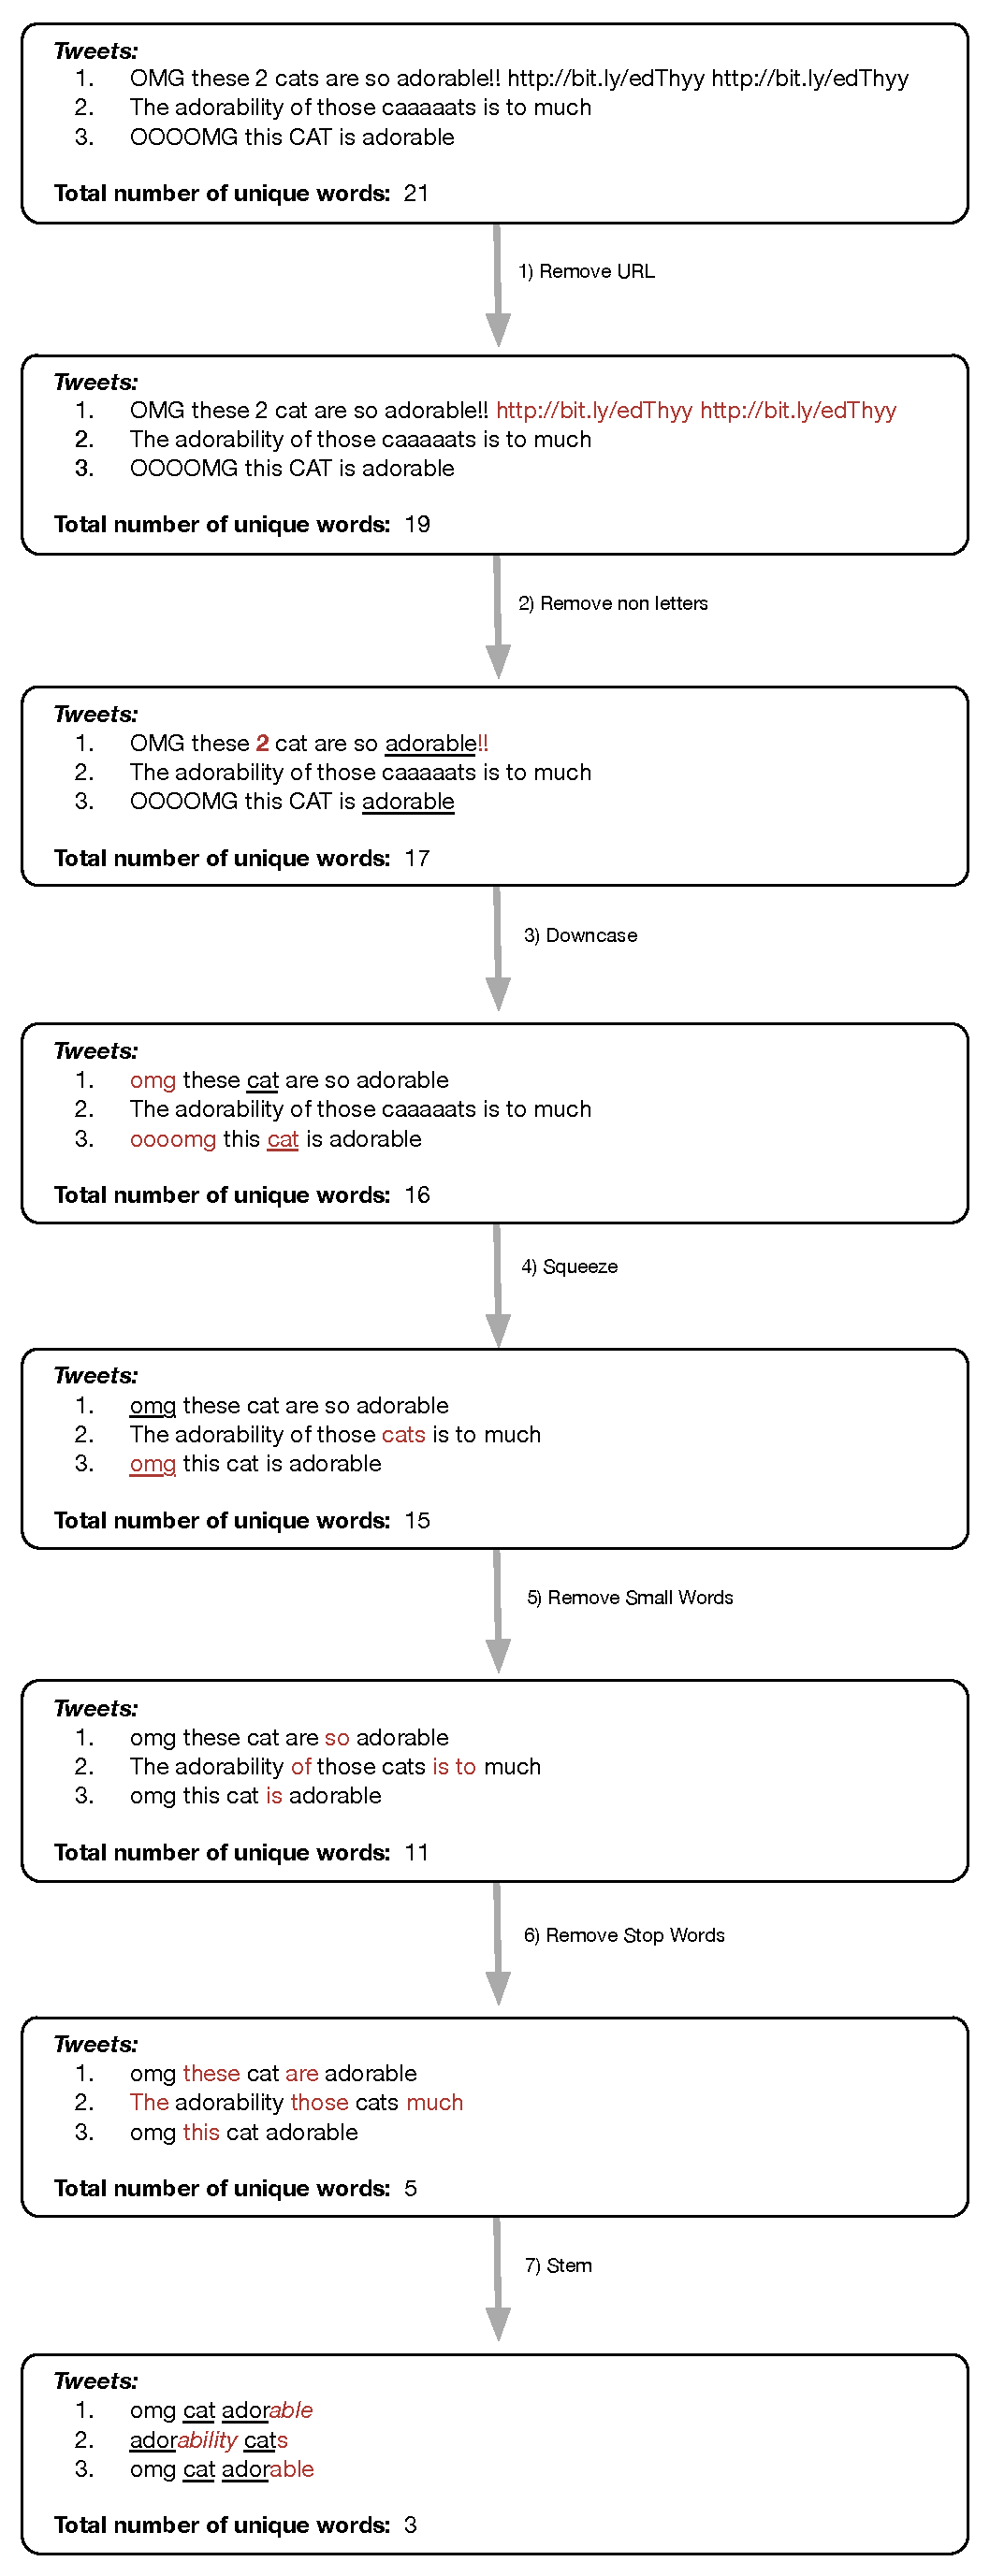
\includegraphics[width=0.8\linewidth]{./images/string_reduction.pdf}
  \caption{Reducing the number of unique words on three tweets about cats. Text in red represents letters removed. Underlined text represents words that due to text transformation became equal.}
  \label{fig:string_reduction}
\end{figure}

Since tweets are very small and have an average of only 10 to 14 words, there is no need to store term frequency on the \ac{VSM}, and therefor only a binary count is made.

\ac{NLP} techniques such as the one described on Subsection~\ref{sub:tweeter_natural_language_processing} can be used in conduction of the method described above for even a more efficient \ac{VSM} reduction. In order to accomplish this, first we need to run the \ac{NLP} on the dataset and specify what kind of tags we want to use. Then, we run the string reduction techniques described above on the words tagged by the \ac{NLP}, these words will then be used to create the \ac{VSM} where each word represents on column. This process can be seen in Figure~\ref{fig:string_nlp}.
\begin{figure}[htpb]
  \centering
  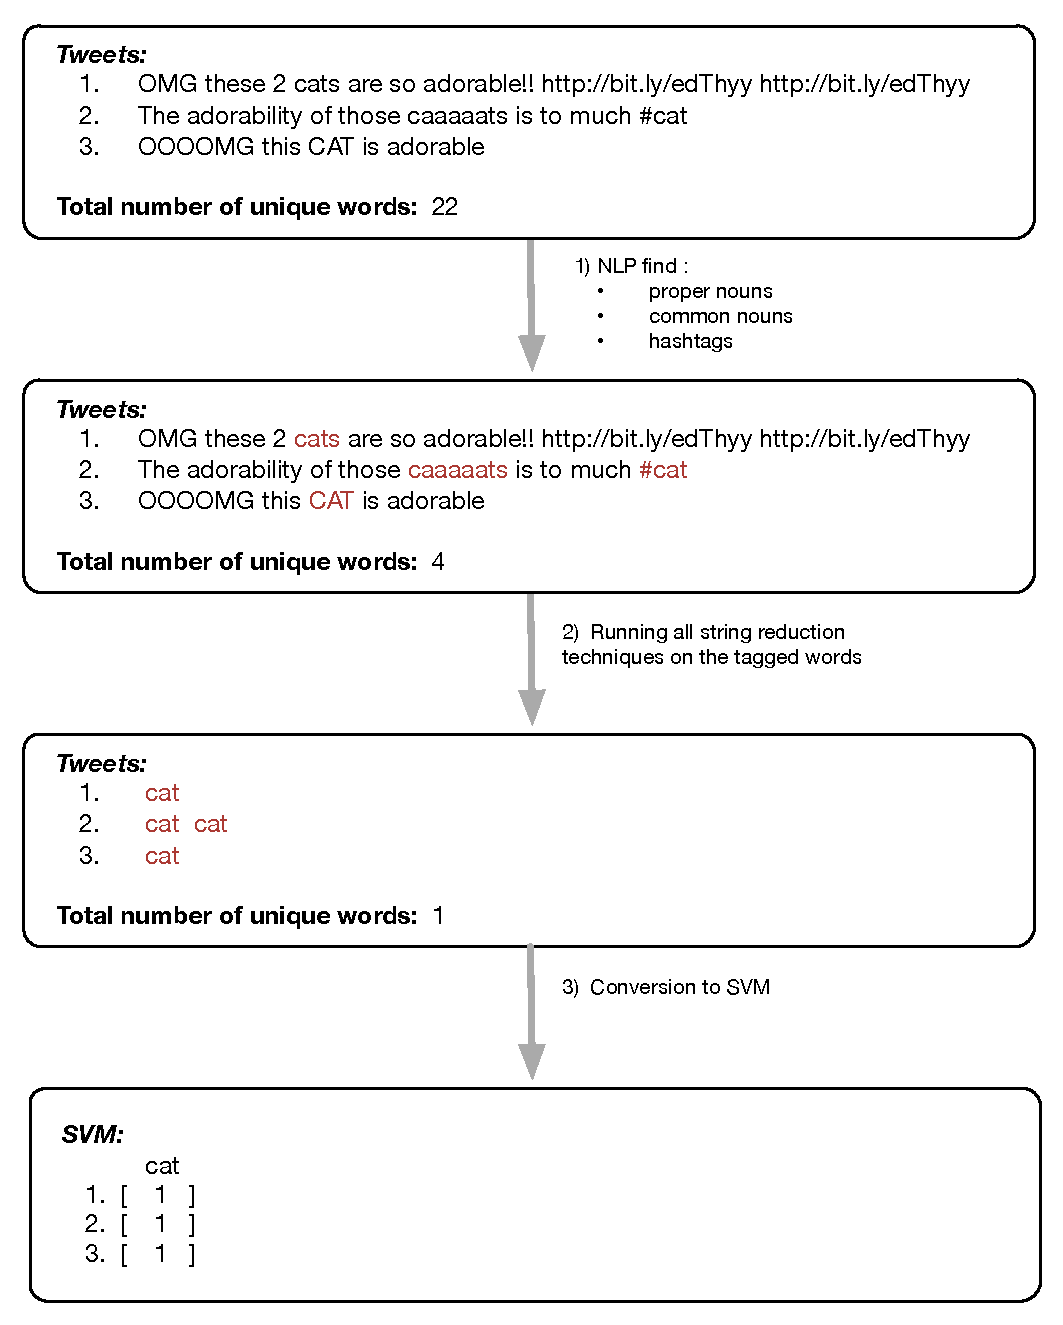
\includegraphics[width=0.8\linewidth]{./images/string_reduction_nlp.pdf}
  \caption{Using NLP with string reduction techniques to reduce the VSM size}
  \label{fig:string_nlp}
\end{figure}

Converting tweets from text to \ac{VSM} can be done in two different approaches. The first one is the cumulative approach, where the \ac{VSM} is being built at the same time that the tweets are read, new terms are added as columns to the \ac{VSM} as soon as they are found. The second way relies on scanning all words present in the dataset in order to first build the \ac{VSM}, then iterate through all tweets and mark them as ones and zeros if they occur in the tweet text. 


After the \ac{VSM} is filled with tweets, it can be feed to the \ac{SOM} and therefor training can start. It is important to notice though, since a destructive process was done to minimize the size of the \ac{VSM} some extra mechanisms must be implemented in order for the tweets to be humanly readable after training.



\subsection{Extensible SOM Library}
\label{sub:extensible_som_library}

When researching ways to extend the \ac{SOM} algorithm, by adding social features to the learning process, we found that there weren't many \ac{SOM} software libraries. Even though, programing languages often used in \ac{ML} and Data Mining, such as Python or C++, have their own implementation of the \ac{SOM} algorithm. We've found that most of these libraries are made in such a way to be extremely fast, in order to take as much advantage from the hardware they are running on as possible. They often lack the modularity needed to adapt the \ac{SOM} algorithm to specific problems.

The \ac{SOM} algorithm has been changed many times in order to better categorize data with specific features. For example, the previously described in Subsection~\ref{sub:types_of_soms} Geo-\ac{SOM}, the Growing Hierarchical \ac{SOM}~\cite[]{1058070}, the time adaptive \ac{SOM}~\cite[]{1187438}, the Ontological \ac{SOM}~\cite[]{5446427}, and the list goes on\dots  

The \ac{SOM} framework is an open source ruby library for creating custom \ac{SOM} implementations. The \ac{SOM} framework, implements the basic \ac{SOM} algorithm with a squared output space, is readably available. Any kind of data which implements enumerable --- can be treated as arrays --- can be used as input patterns. 

It is possible to print \ac{U-Matrix}, \ac{Q-Matrix} at any given time of the training, as well as inspect the topological error. In case the output space is represented as colored vectors, it is also possible to print the current color of the output space at each iteration.

In order to create the homophilic \ac{SOM}, described in Section~\ref{sec:algorithm_changes} we first created a \ac{SOM} framework that is easy to extend due to be fully object oriented, scripted --- even though it can be compiled to run on the JVM --- and without C extensions.


\subsection{Homophilic SOM Definition}
\label{sec:algorithm_changes}
The default \ac{SOM} algorithm has no idea whatsoever of the social connections between the tweets, it simply looks at the binary vectors that represent sentences and assigns it to the most similar neuron.

In order to better categorize socially connected data, we propose some alterations to the \ac{SOM} algorithm in order to make it aware of the social connections between the tweets, and therefor, better represent the homophilic behavior present on social networks.

\subsubsection{Output Space}
\label{sub:output_space}
The output space is the zone on the \ac{SOM} algorithm where the neurons reside. It works like a cortex where neurons are scattered in a geometric fashion, generally a square. The output space is generally initialized with random values, with a relatively high learning rate, and also a relatively high number of epochs. The algorithm is made this way in order to be able to identify any type of data that can be represented as vectors.

First, we will try to change the output space to better resemblance the social network. In order to do this, the squared grid that defines the output space was changed by the social network connections, and the neurons, are represented by a social network user. This changes are applied in the following way:

\begin{figure}[h]
  \centering
  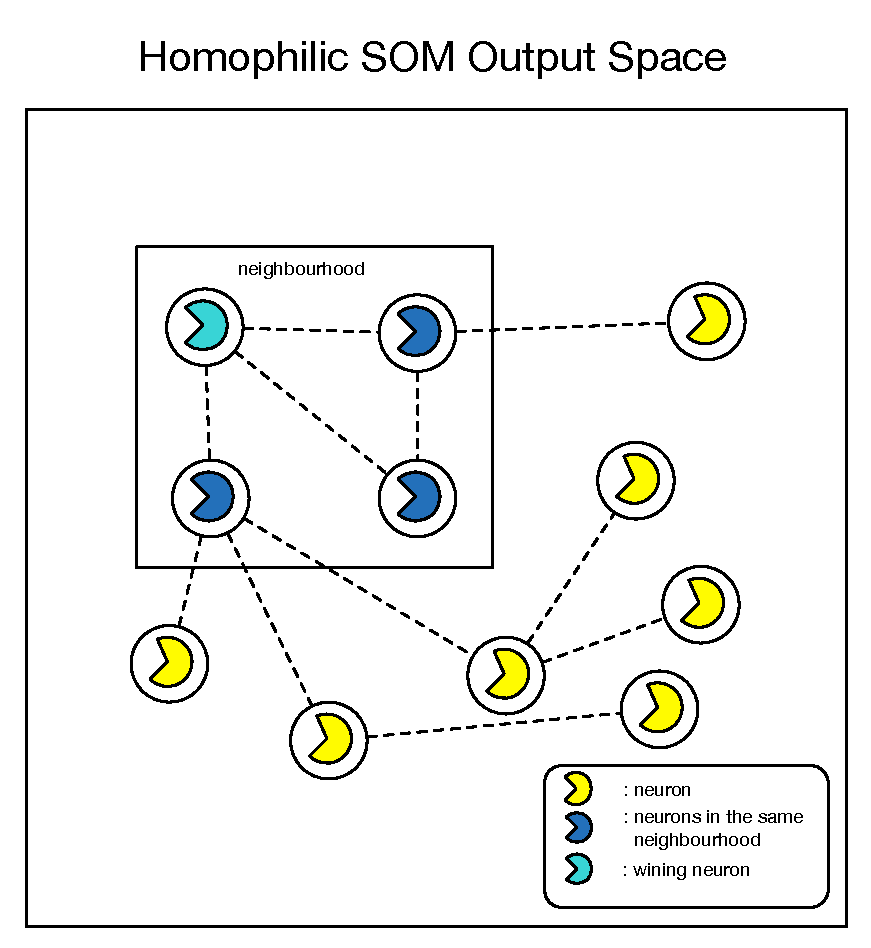
\includegraphics[width=0.6\linewidth]{./images/homophilic_outputspace.pdf}
  \label{chp3:homout}
  \caption{ The neighborhood is defined by the relations of followers/followees between the winning neuron and the other neurons }
\end{figure}

\begin{figure}[h]
  \centering
  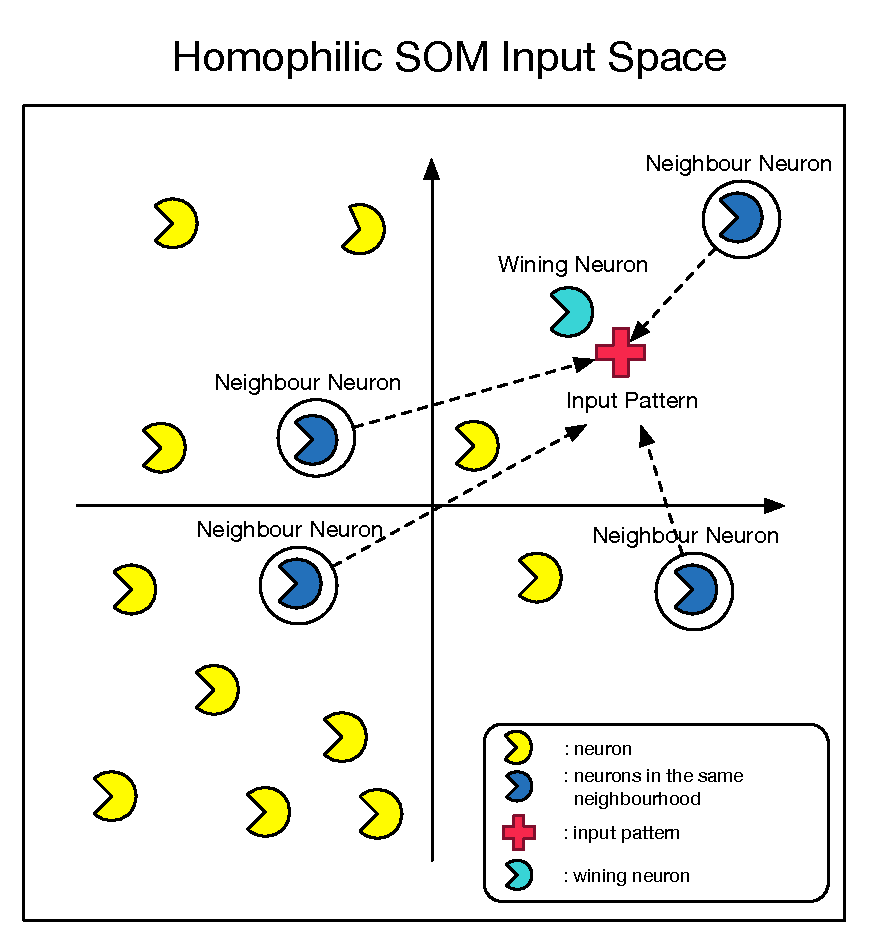
\includegraphics[width=0.6\linewidth]{./images/homophilic_input_space.pdf}
  \label{chp3:homin}
  \caption{ Homophilic input space works in the same way as a normal input space}
\end{figure}

\begin{itemize}
  \item Each neuron is comprised of the text from all the tweets that he authored.
  \item Each neuron has a unique id, and stores the ids of his followers and followees that are present in the output space.
  \item During the learning phase, the radius will be defined as the maximum number of hops separating the winning neuron and followers/followees of followers/followees. 
\end{itemize}


\subsubsection{Learning Phase}
\label{sub:learning_phase}
Like in the default \ac{SOM}, the learning phase is where the output space is trained in order to organize the input data into clusters. Since this algorithm is specific to categorize tweets using social network features, the learning rate, radius and number of epochs used can be greatly reduced in order for the algorithm to converge. The learning phase operates in the following way:

\begin{itemize}
  \item The distance between the input pattern and all the neurons is calculated. The neuron closest to the input pattern is considered the winning neuron.
  \item When the winning neuron is selected, it and its social neighbors within k hops, update their representations in the input space, and move closer to the input pattern. The Gaussian function (Func.~\ref{eq:gaussian}) is also used here. As a way for the neighbors that are closer to the winning neuron, be significantly more influenced by the input pattern, while the neurons further away are less influenced. 
  \item This process is repeated for a predefined number of epochs. In order for the algorithm to converge, whilst the number of epochs increases, the learning rate and number of hops that defines the neighborhood decreases.
\end{itemize}

Just like the default \ac{SOM} algorithm, after the map is trained, input patterns can be fast assign to the nearest neuron since the neuron positions in the output space are no longer updated.
 
\section{Result Assessment}
\label{sec:result_assessment}

\subsection{SOM training}
\label{sub:clustering_tweets_with_soms}
Our first approach to cluster tweets with \ac{SOM} started by dynamically creating \ac{VSM} for each new word that was encountered while scanning each tweet on the dataset. Due to simplicity of the approach, an overwhelming amount of different words, some even without any clear meaning, took relevance on the \ac{VSM}. 
This created a \ac{VSM} with a huge size and the trainings at hand took an eternity to process. In order to prevent this from happening, we took a sample of 50MB of tweets, all in English, from the dataset and started to train the \ac{SOM} with it. String manipulation for \ac{VSM} reduction described on Subsection~\ref{sub:clustering_tweets} were used.
The \ac{SOM} training was performed using the R kohonen package~\cite{rsom}. Three kinds of clusters were found: clusters where no topic could be made sense of, clusters with one or more topics and clusters with a ton of tweets which had the same text .

\subsection{Reducing SOM vector size}
\label{sub:reducing_som_vector_size}
String reducer methods enable great \ac{VSM} reduction. On Figure~\ref{fig:plot_word_red}, we can see the amount of words removed by each method alone, and by all methods combined --- column "All Methods". In order to build this graph, we applied each method independently to a sample of 902802 tweets.

\begin{figure}[h]
  \centering
  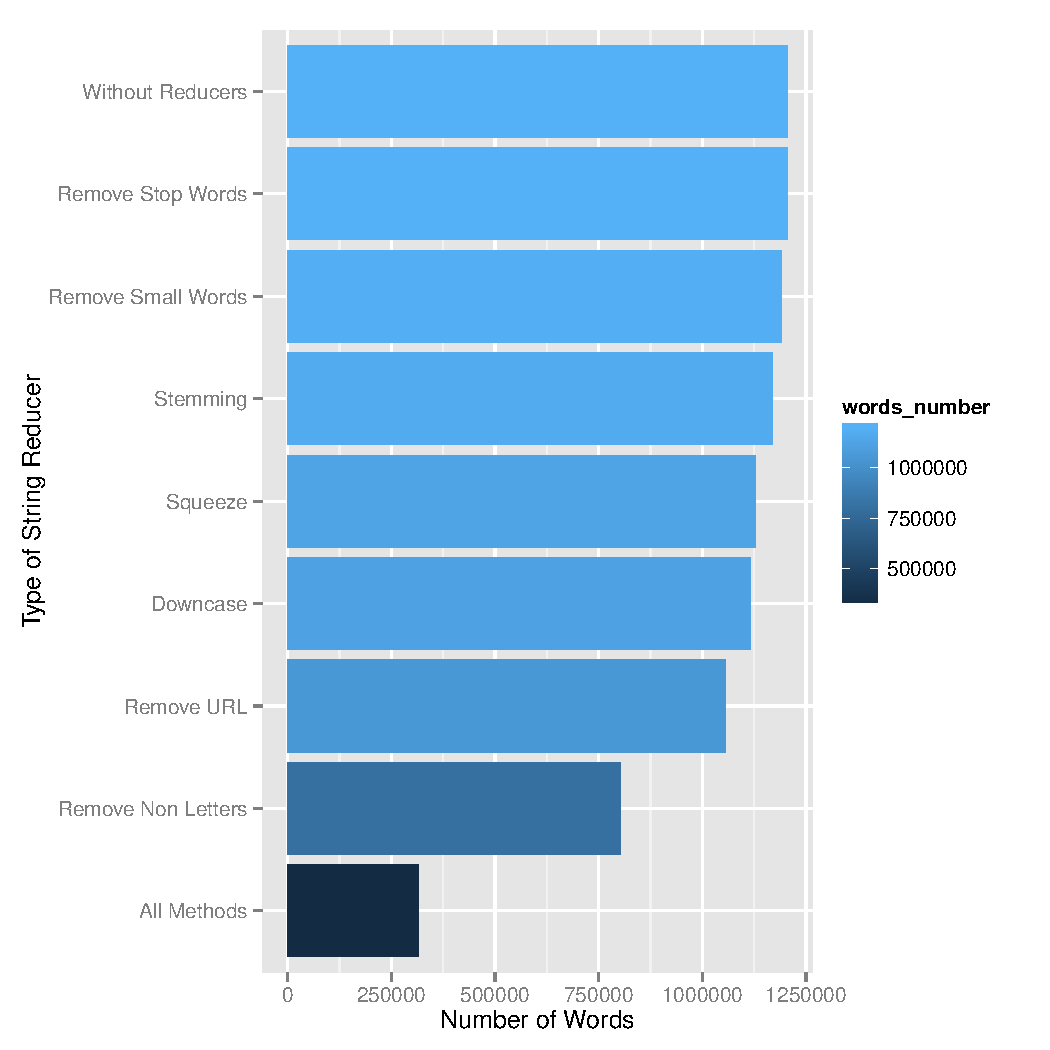
\includegraphics[width=1\linewidth]{./plots/svm/plot_wordcount.pdf}
  \caption{Amount of unique words present on dataset sample with 902802 tweets, based on the string word reduction technique applied.}
  \label{fig:plot_word_red}
\end{figure}

It is interesting to see that each method by itself doesn't remove a great amount of words. The method that removed more words by itself was "remove non letters" --- which removes every character that is not a letter ---, at an order of 33\%. On the other hand, the method "remove stop words" by itself removed only 400 of words. This was expected due to the fact that the full list of MySQL stop words used by this method only has 543 words. All methods combined were able to reduce the \ac{VSM} size in about 75\%.

String reduction techniques work directly with text and has no notion whatsoever of linguistic semantics. 

By feeding the same dataset as used above to the library, we were able to identify multiple types of words that can afterwards be considered relevant for~\ac{TDT}. On Figure~\ref{fig:wordcount_nlp}, the red bars show the amount of unique words found under a specific semantic tag, whilst in blue we can see words tagged under the same category after applying string reduction techniques.

Due to the fact that we are trying to identify topics, most of the tagged words are of no use. We chose to use only common nouns, proper nouns and hashtags during the clustering process. By applying all these filters to the dataset sample, we have a \ac{VSM} reduction of about 90\%, from 1 204 743 different words to 132 861.

\begin{figure}[h]
  \centering
  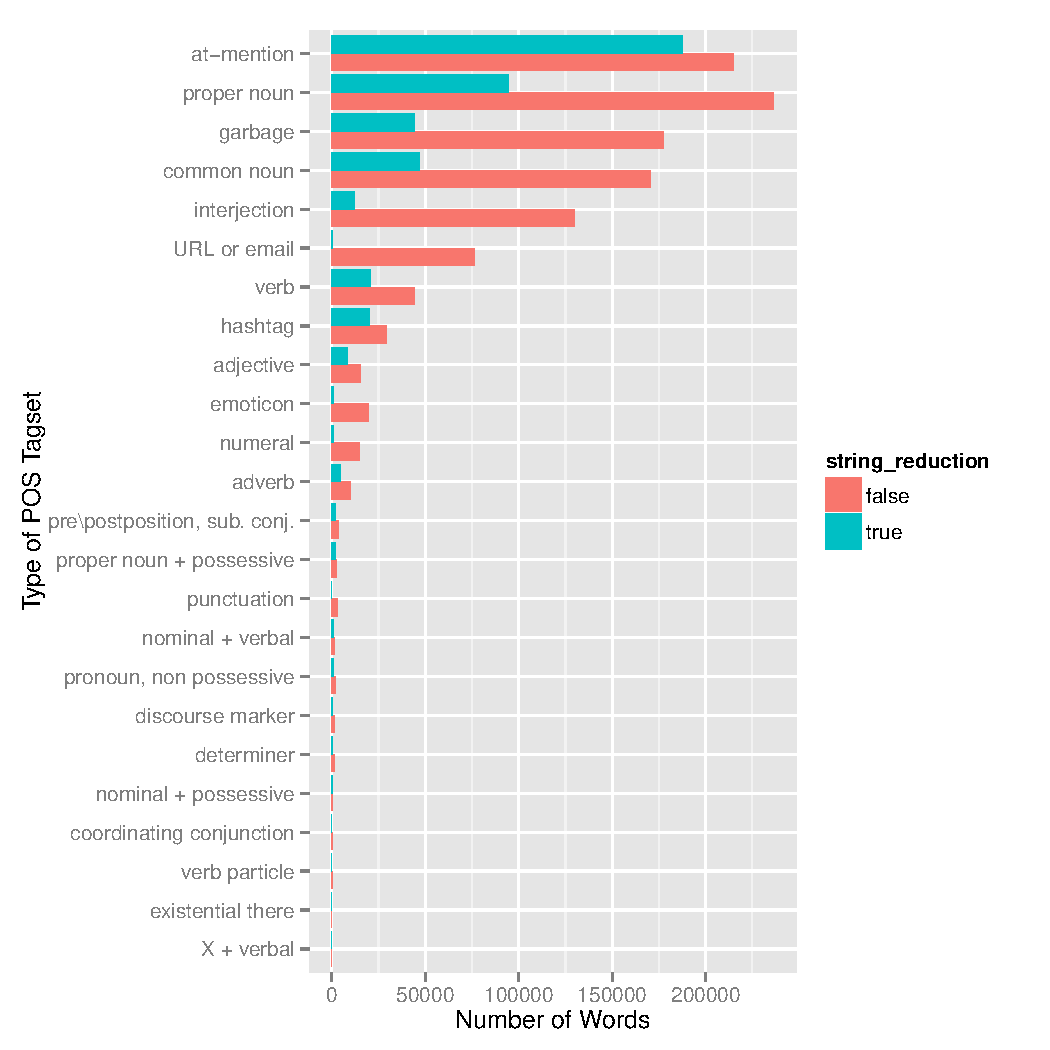
\includegraphics[width=1\linewidth]{./plots/svm/plot_wordcount_nlp.pdf}
  \caption{Number of words tagged with Ark Tweet NLP. In red we can see the number of unique words tagged in each category, while in blue we can see the amount of unique words, after applying string reduction techniques.}
  \label{fig:wordcount_nlp}
\end{figure}

\subsubsection{Identify Tweets language}
\label{sub:identify_tweets_lang}
Twitter is a social network with users from every corner of the world, thus tweets tend to be in a lot of different languages. Twitter internationalization greatly affects the clustering process, with multi language synonyms and idiomatic expressions. Another problem is associated with results interpretation, when a cluster is formed with tweets with languages foreign to the people who are analyzing the results. When this happens, identifying topics on the cluster is extremely hard, and most of the times the researcher will have to manually translate a cluster.  

One way to infer a tweet language, is by looking at the language which a user has on his twitter profile, through the twitter API. Some times, users use their profiles on different languages than the language in which they issue their tweets, which makes the process of excluding foreign tweets harder.

An alternative approach to language identification, is by using an external library like whatlanguage~\footnote{https://github.com/peterc/whatlanguage}, which tries to identify one language through the usage of Bloom Filters.  

In order to better understand the relationship between a tweet language and a user profile language, we analyzed a sample of 87 tweets, all from different users and categorized their language by hand. We found that 7 users were using an English profile, and tweeting in other language.

On the same sample, we used the language identification library and found that even though only 8 tweets were identified as being in English, it did not misidentified any foreign tweet as being in English.

Even though the sample is quite small, it was possible to understand that selecting only tweets with English profiles and afterwards selecting only the ones identified in English by the language identification library, could yield a bigger number of false negatives --- tweets in English which were thought to be in other language ---  , but would help prevent selecting tweets that were not in English.
 
\section{SOM Framework}
\label{sec:som_framework}
The \ac{SOM} framework was developed in the Ruby programing language \footnote{https://www.ruby-lang.org/en/} due to the desired characteristic of allowing great levels of introspection and being an almost pure object oriented programing language. Due to this characteristics, making modifications to core parts of the algorithm is fairly easy.

The \ac{SOM} Framework was developed in a test driven fashion, having 100\% of its public methods tested and documented for expected behavior. These characteristics, associated with the fact that was published under an open source license, makes it available for other researchers to implement their own SOM variants.

By default, the base SOM algorithm is implemented as described by the Algorithm~\ref{alg:som}.
\subsection{Clustering Color Vectors}
\label{sub:main_features}
Out of the box, the \ac{SOM} Framework implements a squared output space, where all residing neurons are manipulated as arrays. It is possible at any given moment of the training to export the output space to \ac{JSON}, \ac{CSV} or to visualize its current \ac{U-Matrix}. Also, during training, a progress bar is displayed in order to know how much time will be needed for the training to end.

Due to the features described above, it is possible to train a \ac{SOM} to identify random colors --- RGB vectors --- while printing the results. In order to do this, we will start by:
\begin{itemize}
  \item Initializing a SOM object with an output space size of 15 by 15 neurons, which will yield a total of 255 neurons --- and directly maps to the maximum number of clusters --- and 700 epochs.
  \item Create 1500 input patterns with size 3 and random values between 0 and 255. 
  \item Tell the SOM to print its state at the end of each epoch.
\end{itemize}

\begin{figure}[h]
  \centering
  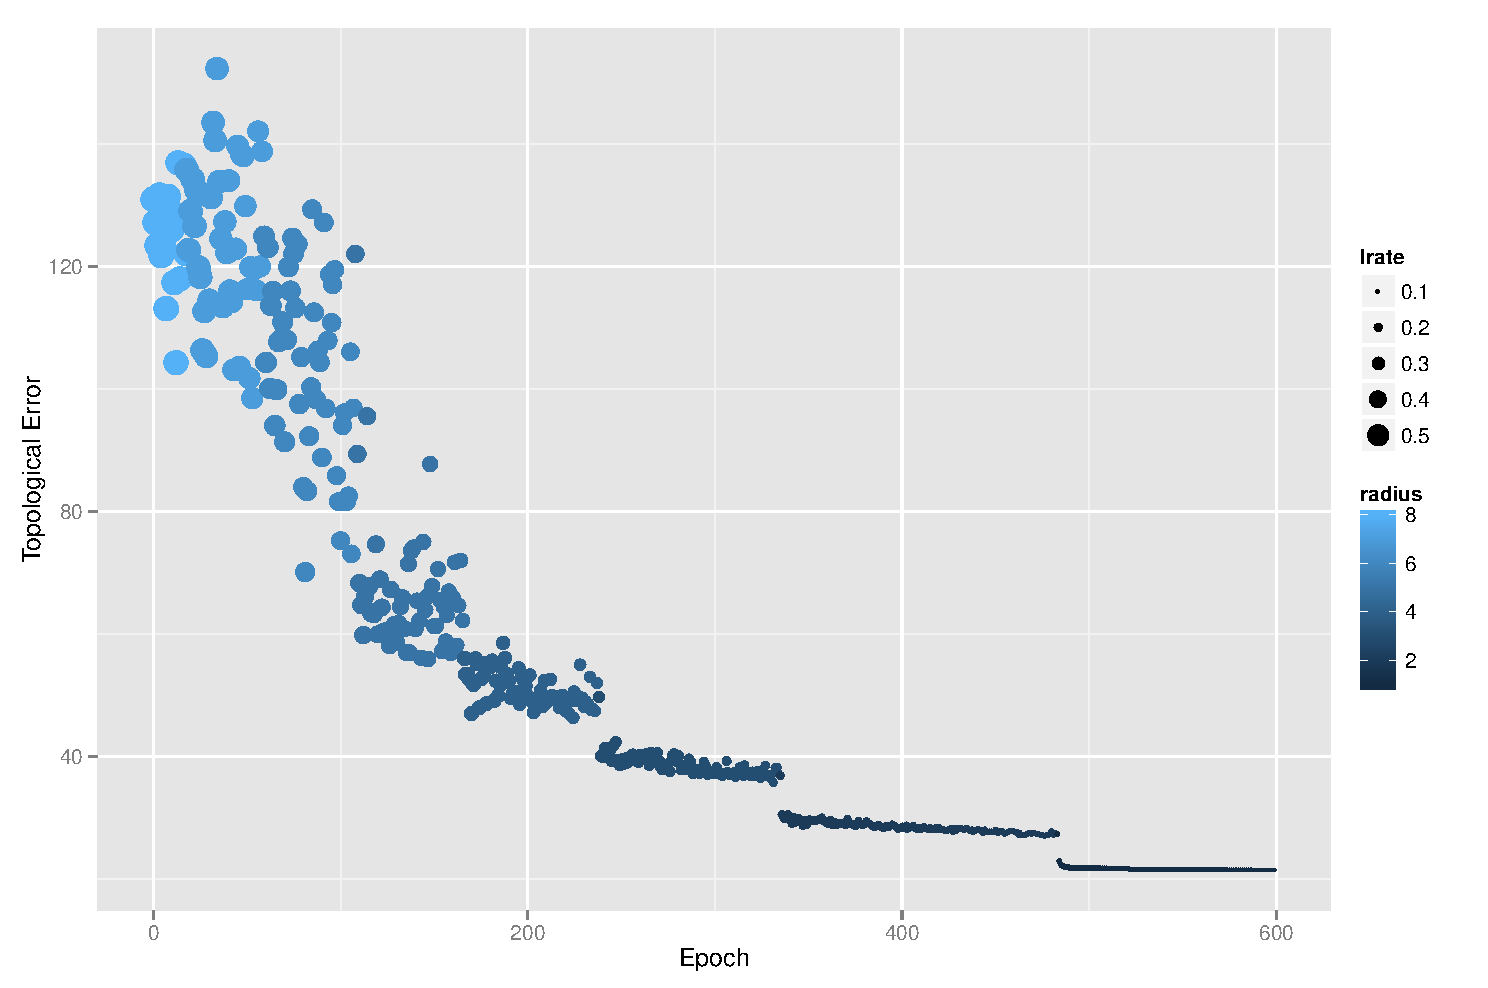
\includegraphics[width=1\linewidth]{./plots/som/topological_error.pdf}
  \caption{Changes in topological error throughout the SOM training, lrate stands for learning rate, and radius for radius applied to the winning neuron}
  \label{fig:top_error}
\end{figure}

On Figure~\ref{fig:top_error} we can see the evolution of the topological error and how it is converging throwout the training process, as the radius and learning rate are decreasing, and as well as the number of epochs is rising. 

\begin{figure}[h]
  \centering
  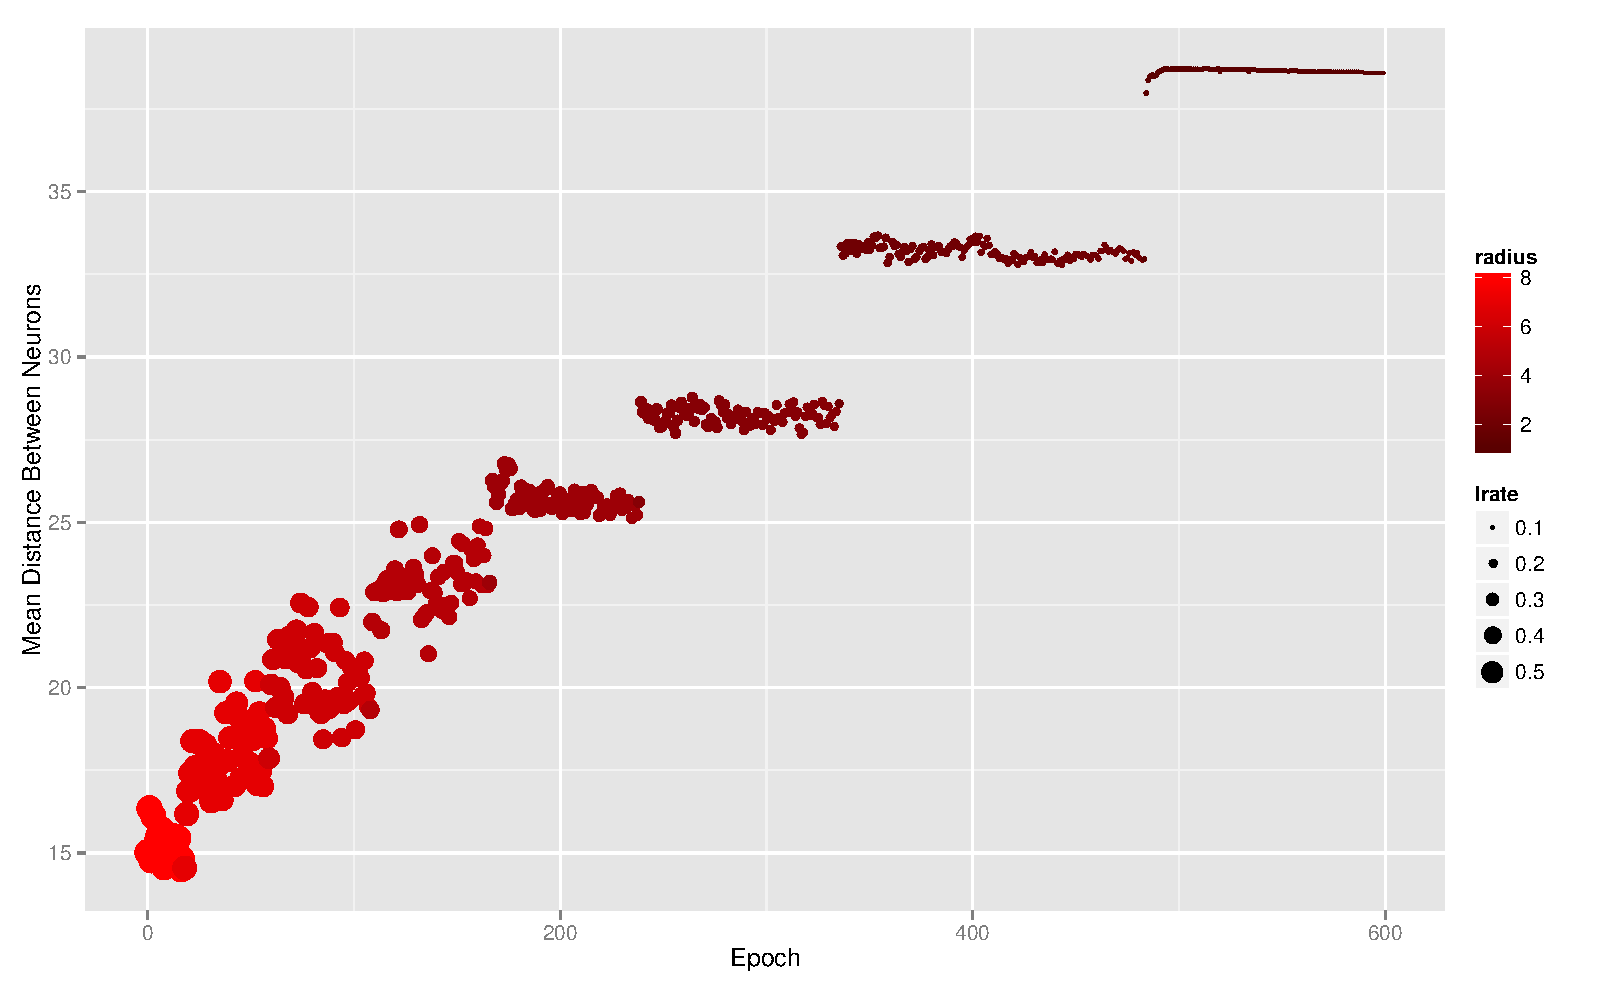
\includegraphics[width=1\linewidth]{./plots/som/average_distance.pdf}
  \caption{Changes in the average distance between neurons, throughout the SOM training}
  \label{avg_dist}
\end{figure}

On Figure~\ref{avg_dist} we can see the average distance between neurons increasing. At first this might not look like a desired property, but in fact it is. When the distance between the neurons is increasing and the topological error is decreasing, it means that the neurons are scattering in the output space in order to better identify the input patterns they are responsible for.

During the training of this \ac{SOM}, we analyzed the output space, \ac{U-Matrix} and \ac{Q-Matrix} during the begging, half of the train, and finally at the end of the training.
The \ac{U-Matrix} evolves in a way where clusters are almost unnoticeable, which is caused by the homogeneity and randomness of the input patterns. 
The \ac{Q-Matrix} evolves, by becoming whiter which represents that the mean topographic error is becoming smaller. This was already seen before in Figure~\ref{fig:top_error}, but now we can also see which neurons are worst at representing the input patterns.  
%\begin{figure}[h]
 %\centering
  %\mbox{\subfloat[]{\label{chp3:threesom} 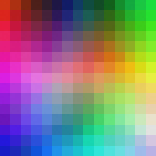
\includegraphics[width=0.8\linewidth]{./images/som_training/3_som.pdf}}}
  %\mbox{\subfloat[]{\label{chp3:threematrix} 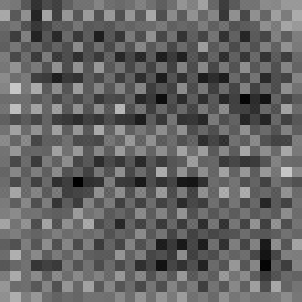
\includegraphics[width=0.8\linewidth]{./images/som_training/3_umatrix.pdf}}}
  %\mbox{\subfloat[]{\label{chp3:threetopmat} 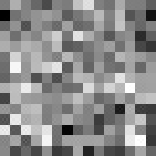
\includegraphics[width=0.8\linewidth]{./images/som_training/3_quantmatrix.pdf}}}
%\end{figure}

\begin{figure}[h!]
  \centering
  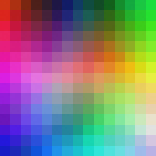
\includegraphics[width=0.4\linewidth]{./images/som_training/3_som.pdf}
  \caption{Output Space, at the end of training.}
  \label{chp3:threesom}
\end{figure}

\begin{figure}[h!]
  \centering
  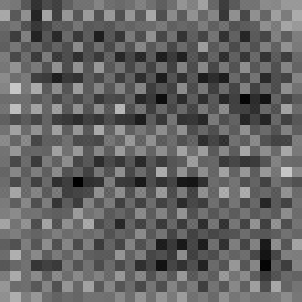
\includegraphics[width=0.4\linewidth]{./images/som_training/3_umatrix.pdf}
  \caption{U-Matrix, at the end of training.}
  \label{chp3:threematrix}
\end{figure}

\begin{figure}[h!]
  \centering
  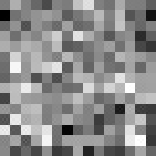
\includegraphics[width=0.4\linewidth]{./images/som_training/3_quantmatrix.pdf}
  \caption{ Q-Matrix, at the end of training.}
  \label{chp3:threetopmat}
\end{figure}
 
In order to see how well the neurons are representing the input patterns, we looked at the \ac{Q-Matrix} and selected the darkest area in order to know which neuron is the worst at representing its input patterns. Afterwards, we printed the input patterns associated to that neuron. This process was graphically represented in Figure~\ref{fig:somtrained} where the colors which represent the input patterns are in fact RGB vector coordinates used during training. It is possible to see that even though this neuron ought to be the worst at representing it input data, he represents it quite well as they are all shades of red. 
It is important to know that all of this visualization can only be made due to the fact that, we are working with arrays with three dimension and values comprised between 0 and 255 --- which makes it possible for them to be presented as RGB images. 

\begin{figure}[h!]
  \centering
  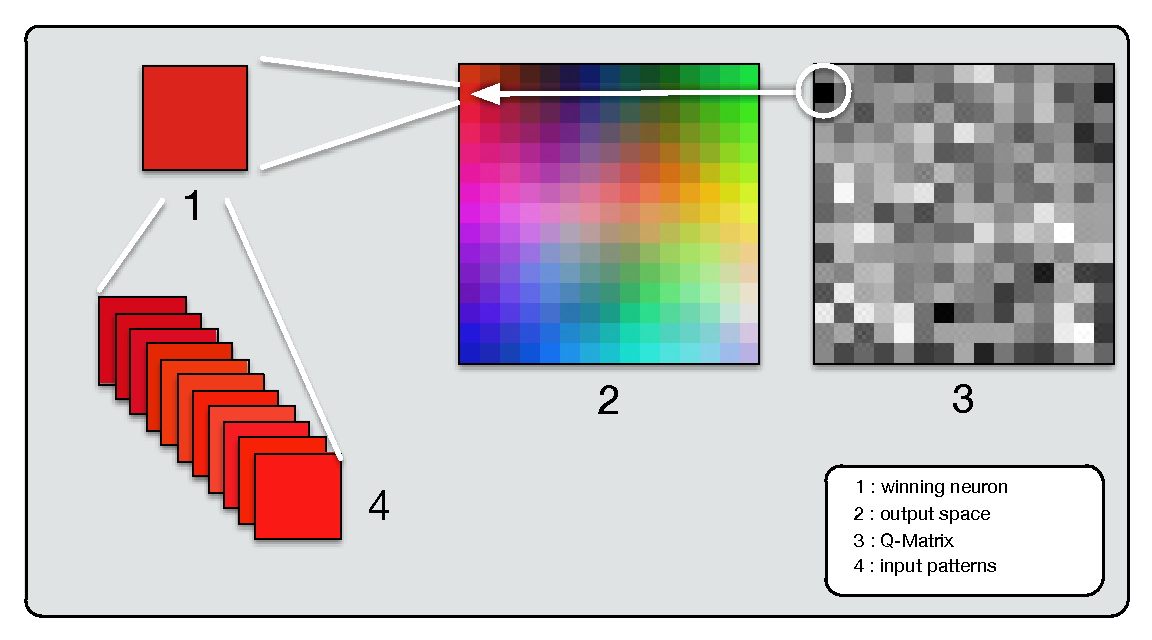
\includegraphics[width=1\linewidth]{./images/som_trainned.pdf}
  \caption{Input patterns associated with the neuron with maximum topological error --31. Even though the neuron has the biggest topological error of all neurons, it still has a good representation of the input patterns. The colors in this image are not figurative, and represent the entities at the end of training.  }
  \label{fig:somtrained}
\end{figure}

\subsection{Benchmarking}
\label{sub:benchmarking}
The \ac{SOM} framework was not created with the purpose of being extremely fast, for that there are already very good implementations like \citet{somoclu} distributed library for \ac{SOM} or \citet{rsom} R kohonen package which implements the training algorithm in C, and only exposes the interface in the high level language R.  
Being purely written in a higher level language, the \ac{SOM} framework enables researchers and programmers to write training algorithms very fast. 

The framework was tested against multiple sizes of output space and input patterns, multiple numbers of input patterns, and multiple numbers of epochs. 
The results were summarized on Figure~\ref{fig:benchmarkingsom}, where it is possible to see on the upper quadrant that if all parameters increase, \ac{SOM} training will suffer as well.

\begin{figure}[h]
  \centering
  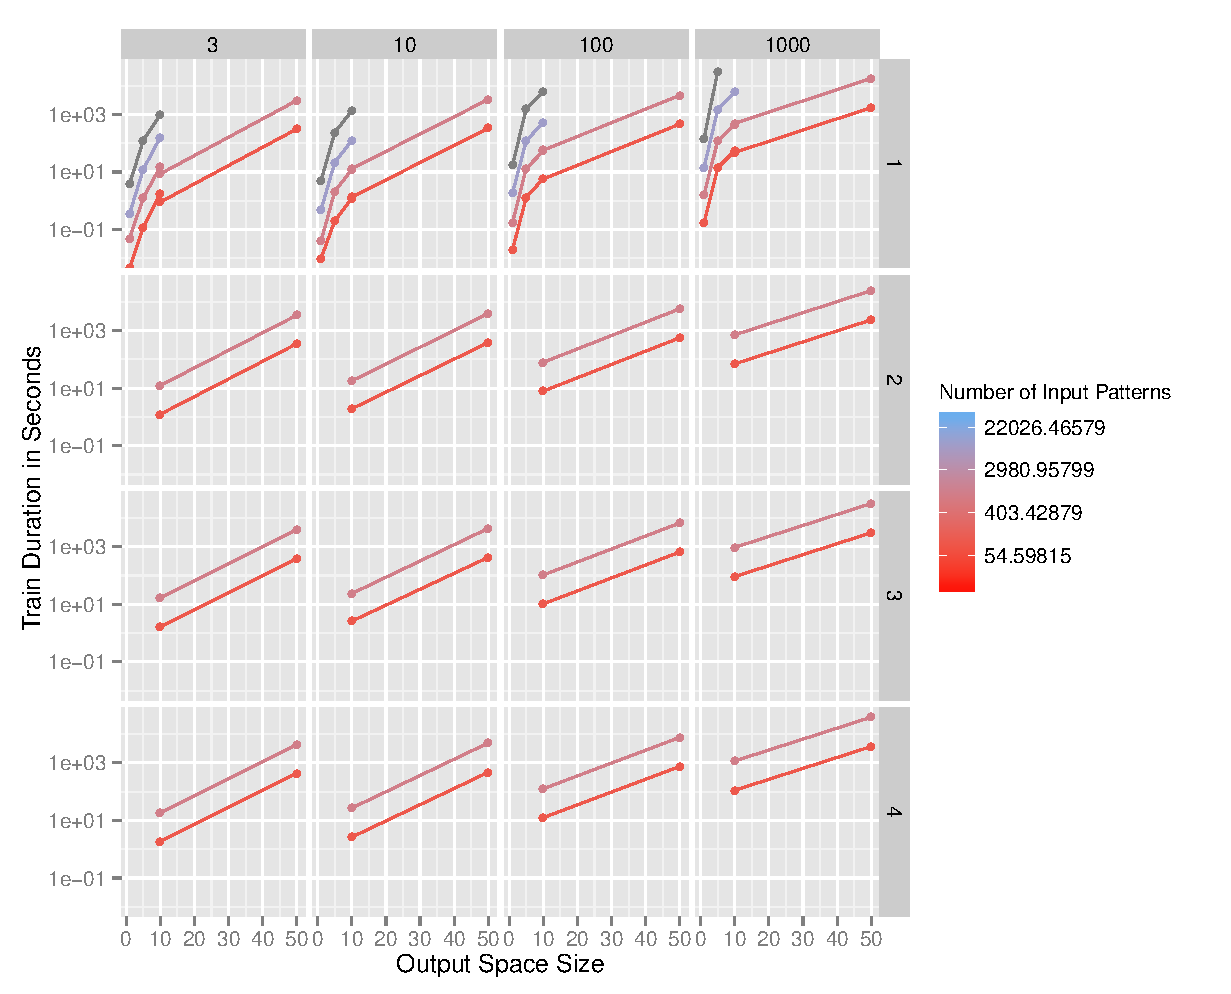
\includegraphics[width=1\linewidth]{./plots/som/benchmarking.pdf}
  \caption{SOM framework train duration, influenced by output space size in the XX axis, duration of the training on the YY axis, number of epochs in the right, size of input patterns on top, and number of input patterns on the right in color from red to blue.}
  \label{fig:benchmarkingsom}
\end{figure}

\subsection{Homophilic SOM}
\label{sec:homophilic_som}
In order bring the concept of homophily --- which have proved to be present on social networks~\cite[]{Wehrens2007}  --- to clustering socially connected data, on Section \ref{sec:algorithm_changes} we suggested some alterations to the default \ac{SOM} algorithm. These modifications were mainly applied to the output space, where each neuron started to represent a user, and his neighborhood is comprised of his social relations.

These features were implemented into the \ac{SOM} framework described in the previous chapter.

It is not possible to draw a \ac{U-Matrix} due to the fact that the output space is no longer a rectangular matrix, but a graph. Also drawing, the \ac{Q-Matrix} is possible, but the disposition of the neurons will not represent the actual disposition in the graph. This can still be useful to easily visualize which neurons are better at representing their input patterns. 

Looking at the results, there are a lot of different topics of clusters. There were neurons clearly responsible to identify music, clusters about tech and programing which surprisingly could identify the tweet about the banana phone which was tech project presented at codebits. These clusters can be seen in Figure~\ref{clust:tech} and ~\ref{clust:music}.
On the other hand, some clusters of people saying that they have posted photos on facebook, or that they've liked youtube videos were also found. Even though they can be considered topics, their relevance is not very high.

\begin{figure}[h]
  \centering
  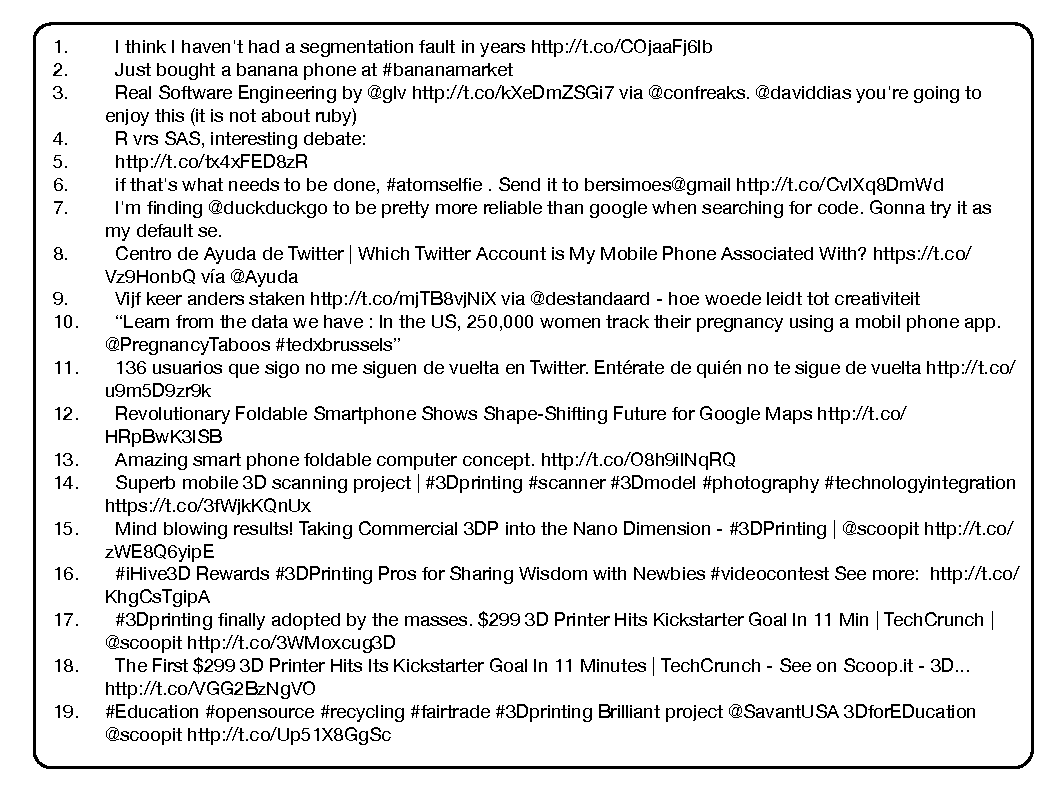
\includegraphics[width=0.8\linewidth]{./images/1clustertech.pdf}
  \label{clust:tech}
  \caption{Cluster about tech and programing}
\end{figure}

\begin{figure}[h]
  \centering
  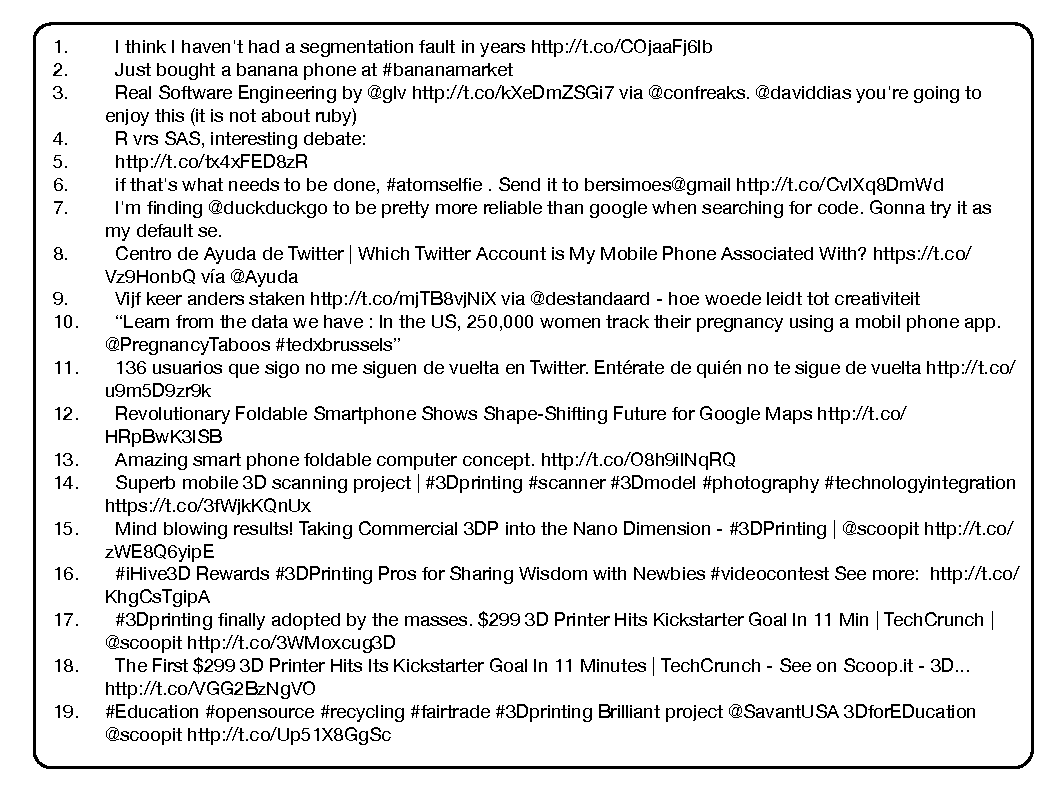
\includegraphics[width=0.8\linewidth]{./images/2clustertech.pdf}
  \label{clust:music}
  \caption{Cluster about music}
\end{figure}
               
\section{Conclusions and Future Work}
This work presents an innovative approach to topic detection on social networks. The clustering mechanism takes into consideration the concept of homophily, which have been proved to occur in social  networks~\cite{Wehrens2007}.
In order to achieve this, we presented a new way to reduce the \ac{VSM} up to 90\% with minimum relevant data loss for topic detection on twitter. Built a \ac{SOM} library in ruby,  which we edited afterwards to add social connections to the neurons during the training process.

Proposed a new visualization technique for \ac{SOM} called \ac{Q-Matrix}, where it is possible to see how well a neuron represents its associated input patterns.

As future work, we would like to improve performance of Homophilic \ac{SOM} in order for it to be able to crunch a lot more data. It would also be awesome to have some pre categorized tweets, so we could compare results faster without having to be reading the content of the clusters.

Also designing \ac{U-Matrix} and \ac{Q-Matrix} for the homophilic \ac{SOM} should be possible. This should be accomplished, by printing the output space as graph and afterwards,  apply the same concepts used for the squared output space. One way to do this, would be by processing the \ac{SOM} results into HTML documents, and use libraries like D3js \footnote{http://d3js.org/} to build all the graphical parts. 

               
\bibliographystyle{apalike}
\bibliography{./bibliographies/library,./bibliographies/sites}
\begin{acronym}[TDMA]
	\acro{YAML}{Yet Another Markup Language}
	\acro{SOM}{Self-Organizing Maps}
	\acro{DC}{Document Clustering}
	\acro{NLP}{Natural Language Processing}
	\acro{Q-Matrix}{Unified Mean Quantization Error Matrix}
	\acro{U-Matrix}{Unified Distance Matrix}
	\acro{TF-IDF}{Term Frequency–Inverse Document Frequency}
	\acro{BMU}{Best Matching Unit}
	\acro{LDA}{Latent Dirichlet Allocation}
	\acro{TDT}{Topic Detection and Tracking}
	\acro{VSM}{Vector Space Model}
	\acro{IR}{Information Retrieval}
	\acro{ML}{Machine Learning}
	\acro{ANN}{Artificial Neural Network}
	\acro{MDS}{Multi Dimensional Scalling}
	\acro{PCA}{Principle Component Analysis}
	\acro{URL}{Uniform Resource Locator}
	\acro{JSON}{JavaScript Object Notation}
	\acro{CSV}{Comma Separated Values}
	\acro{VM}{Virtual Machine}
	\acrodefplural{SOM}[SOMs]{Self Organizing Maps}
	\acrodefplural{ANN}[ANNs]{Artificial Neural Networks}
\end{acronym}
\end{document}


